\begin{frame}

\frametitle{Conceptos Previos}

\begin{block}{Conceptos Previos}
\begin{itemize}
	\item Optimización Global.
	\item Meta-heuristicas.
\end{itemize}
\end{block}
\end{frame}

%++++++++++++++++++++++++++++++++++++++++++++++++++++++++++++++++++++++++++++++  
\begin{frame}

\frametitle{Optimización Global}

\begin{block}{Definición}
Optimizar una función $f$ dentro de un intervalo especificado.
\end{block}

\begin{block}{Definición Formal}
El objetivo de la optimización global, considerando un problema de minimización, es encontrar un vector $X* \in \Omega$ tal que $f(X*) \leq f(X)$ para todo $X \in \Omega$, donde $\Omega$ es el espacio de búsqueda delimitado por un límite inferior $lb$ y un límite superior $ub$ \cite{Segredo}.
\end{block}
\end{frame}

%++++++++++++++++++++++++++++++++++++++++++++++++++++++++++++++++++++++++++++++


\begin{frame}
\frametitle{Meta-heuristicas}
\begin{figure}
  \centering
	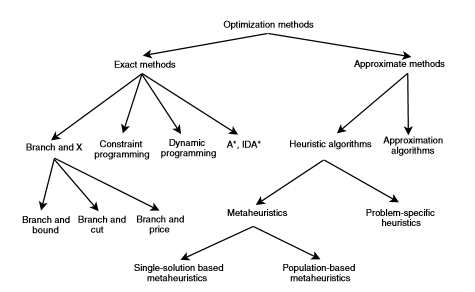
\includegraphics[scale=0.9]{img/meta}\\[10mm]
\end{figure}
\end{frame}

%++++++++++++++++++++++++++++++++++++++++++++++++++++++++++++++++++++++++++++++ 
\begin{frame}

\frametitle{Meta-heuristicas}

\begin{block}{Características}
\begin{itemize}
	\item Soluciones factibles en tiempo aceptable.
	\item Eficiencia y eficacia.
	\end{itemize}
\end{block}

\end{frame}

%++++++++++++++++++++++++++++++++++++++++++++++++++++++++++++++++++++++++++++++
\begin{frame}
\frametitle{Meta-heuristicas}
\begin{block}{Categorías}
\begin{itemize}
    \item \textbf{Búsquedas Locales}: Greedy Randomized Adaptive Search Procedure (GRASP) \cite{GRASP}, Variable Neighborhood Search (VNS) \cite{vns}.
    \item \textbf{Heurísticas Voraces}: Simulated Annealing (SA) \cite{SA}.
    \item \textbf{Algoritmos Evolutivos}: Covariance Matrix Adaptation Evolutionary Strategy (CMA-ES) \cite{CMA}, Differential Evolution (DE) \cite{DE1, DE2, DE3}, Coevolutionary Algorithms (CEA) \cite{COE1, COE2, COE3}.
\end{itemize}
\end{block}
\end{frame}

%++++++++++++++++++++++++++++++++++++++++++++++++++++++++++++++++++++++++++++++
\begin{frame}
\frametitle{Meta-heuristicas}
\begin{block}{Criterios de Diseño}
\begin{itemize}
	\item Intensificación.
	\item Diversificación.
	\end{itemize}
\end{block}
\begin{block}{}
\begin{itemize}
	\item Representación.
	\item Condición de parada.
	\end{itemize}
\end{block}
\end{frame}

%++++++++++++++++++++++++++++++++++++++++++++++++++++++++++++++++++++++++++++++
\begin{frame}[allowframebreaks]
\frametitle{Meta-heuristicas}
\begin{block}{Representación.}
\begin{itemize}
    \item \textbf{Cadena binaria}.
    \begin{figure}[!ht]
    \centering
    
\includegraphics[scale=1.2]{img/binaria}
    \end{figure} 
    \item \textbf{Vector de valores naturales}.
    \begin{figure}[!ht]
    \centering
    
\includegraphics[scale=1.2]{img/natural}
    \end{figure}
\end{itemize}
\end{block}
\end{frame}
\begin{frame}[allowframebreaks]
\frametitle{Meta-heuristicas}
\begin{block}{Representación.}
\begin{itemize}
    \item \textbf{Vector de números reales}.
    \begin{figure}[!ht]
    \centering
    
\includegraphics[scale=1.2]{img/reales}
    \end{figure}
    \item \textbf{Permutaciones}.
    \begin{figure}[!ht]
    \centering
    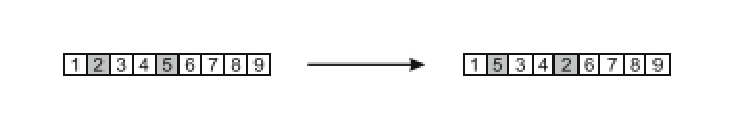
\includegraphics[scale=0.8]{img/secuencia}
    \end{figure}
\end{itemize}
\end{block}
\end{frame}

%++++++++++++++++++++++++++++++++++++++++++++++++++++++++++++++++++++++++++++++
\begin{frame}
\frametitle{Meta-heuristicas}
\begin{block}{Condición de Parada}
\begin{itemize}
    \item \textbf{Iteraciones}.
    \item \textbf{Evaluaciones}.
    \item \textbf{Factor de error}.
\end{itemize}
\end{block}
\begin{block}{}
En nuestro trabajo, el criterio de parada utilizado por todos los algoritmos desarrollados es \textbf{$10^{6}$ evaluaciones}, criterio prefijado por la organización del concurso GenOpt. 
\end{block}
\end{frame}
